\section{Die stabile- und instabile Mannigfaltigkeit und die Smale-Bedingung}

\begin{definition}[Stabile- und instabile Mannigfaltigkeit]
    \label{def: stabile und instabile mannigfaltigkeit}
    Es sei $f \colon M \to \R$ eine Morse-Funktion, $p$ ein kritischer Punkt von $f$ und $X$ ein
    Pseudo-Gradientenfeld von $f$. Die stabile Mannigfaltigkeit von $p$ ist die Menge
    \[ \stab (p) = \left\{ q \in M : \lim_{t \to + \infty} \phi_t(q) = p \right\} \]
    und die instabile Mannigfltigkeit ist
    \[ \unst (p) = \left\{ q \in M : \lim_{t \to - \infty} \phi_t(q) = p \right\} . \]
\end{definition}

Bevor wir die stabile- und instabile Mannigfaltigkeit eines kritischen Punktes weiter untersuchen, 
fixieren wir ein Paar Notationen zu Morse Umgebungen. Für das gesamte Kapitel ist diese Vorstellung
von Morse-Umgebungen wichtig.

\begin{definition}[Notationen zu Morse Umgebungen]
    \label{def: notation morse umgebung}
    Zuerst untersuchen wir eine quadratische Formin $\R^n$, die die Form hat wie Funktionen in Morse
    Umgebungen, also $Q \colon \R^n \to \R$ mit
    \[ Q(x_1, \dots, x_n) = - x_1^2 - \dots - x_k^2 + x_{k + 1}^2 + \dots + x_n^2 \]
    für ein $1 \leq k \leq n$.
    Mit $x_- := (x_1, \dots x_k)$ und $x_+ := (x_{k + 1} \dots x_n)$ gilt dann
    \[ Q = - \| x_- \|^2 + \| x_+ \|^2 . \]
    Der Gradient von $Q$ ist mit dem Standardskalarprodukt auf $\R^n$
    \[ \grad Q (x_-, x_+) = 2(x_-, x_+) . \]
    Es seien $\eps, \eta > 0$. Dann definiere die Menge
    \[ U(\eps, \eta) := \left\{ x \in \R^n : - \eps \leq Q(x) \leq \eps 
    \text{ und } \| x_- \|^2 \| x_+ \|^2 \leq \eta(\eps + \eta) \right\} := U . \]
    Wir definieren außerdem
    \begin{align*}
        \del_{\pm} U := & \left\{ x \in U: Q(x) = \pm \eps \text{ und } \|x_{\mp} \|^2 \leq \eta \right\} 
            \text{ und} \\
        \del_0 U := & \left\{ x \in \del U: \| x_- \|^2 \| x_+ \|^2 = \eta(\eps + \eta) \right\} .
    \end{align*}
    Dann setzt sich der Rand von $U$ aus diesen drei Teilen zusammen, also
    \[ \del U = \del_+ \cup \del_- \cup \del_0 . \]
    $\del_0 U$ ist parallel zu den Trajektorien des negativen Gradienten von $Q$. $\del_+ U$ und 
    $\del_- U$ sind orthogonal zu den Trajektorien des negativen Gradienten von $Q$, wobei die 
    Trajektorien in $\del_+ U$ in die Menge $U$ eintreten und sie in $\del_- U$ wieder verlassen. 
    Wir setzen nun $V_- = \langle e_1, \dots, e_k \rangle$ und 
    $V_+ = \langle e_1, \dots, e_n \rangle \subseteq \R^n$. $V_+$ ist der größte Vektorraum, 
    auf dem $\opd^2 Q (0) (\cdot, \cdot)$ positiv definit ist und $V_-$ der größte Vektorraum, auf dem 
    $\opd^2 Q (0) (\cdot, \cdot) (0)$ negativ definit ist. 
    Es gilt 
    \[ \del U \cap V_{\pm} \subseteq \del_{\pm} U . \]
    $0$ ist der einzige kritische Punkt von $Q$ und ist offensichtlich nicht degeneriert. Damit ist $Q$
    eine Morse Funktion und es gilt 
    $\stab (0) = V_+$ und $\unst (0) = V_-$.

    Ist nun $f \colon M \to \R$ eine Morse Funktion, $p$ ein kritischer Punkt von $f$ und $(V, \psi)$
    eine Morse Umgebung von $p$, dann gilt $f \circ \psi^{-1} = Q + f(p)$. Sind $\eps$ und $\eta$
    klein genug, dann ist $U \subset \psi(V)$. Wir nennen 
    $\Omega (p, \eps, \eta) = \Omega (p) = \psi^{-1}(U)$, und 
    $\del_{\pm} \Omega (p) = \psi^{-1}(\del_{\pm}U)$ und $\del_0 \Omega (p) = \psi^{-1} (\del_0 U)$.
    Dann ist 
    \[ \psi(\stab (p) \cap \Omega (p)) = V^+ \cap U \] 
    und 
    \[ \psi(\unst (p) \cap \Omega (p)) = V^- \cap U . \]
    Wir können uns also mit dieser Notation die stabile- und instabile Mannigfaltigkeit (wenigstens 
    in einer Umgebung von $p$) sehr gut vorstellen.

    \begin{figure}[ht]
        \centering
        \begin{minipage}{.4\textwidth}
          \centering
          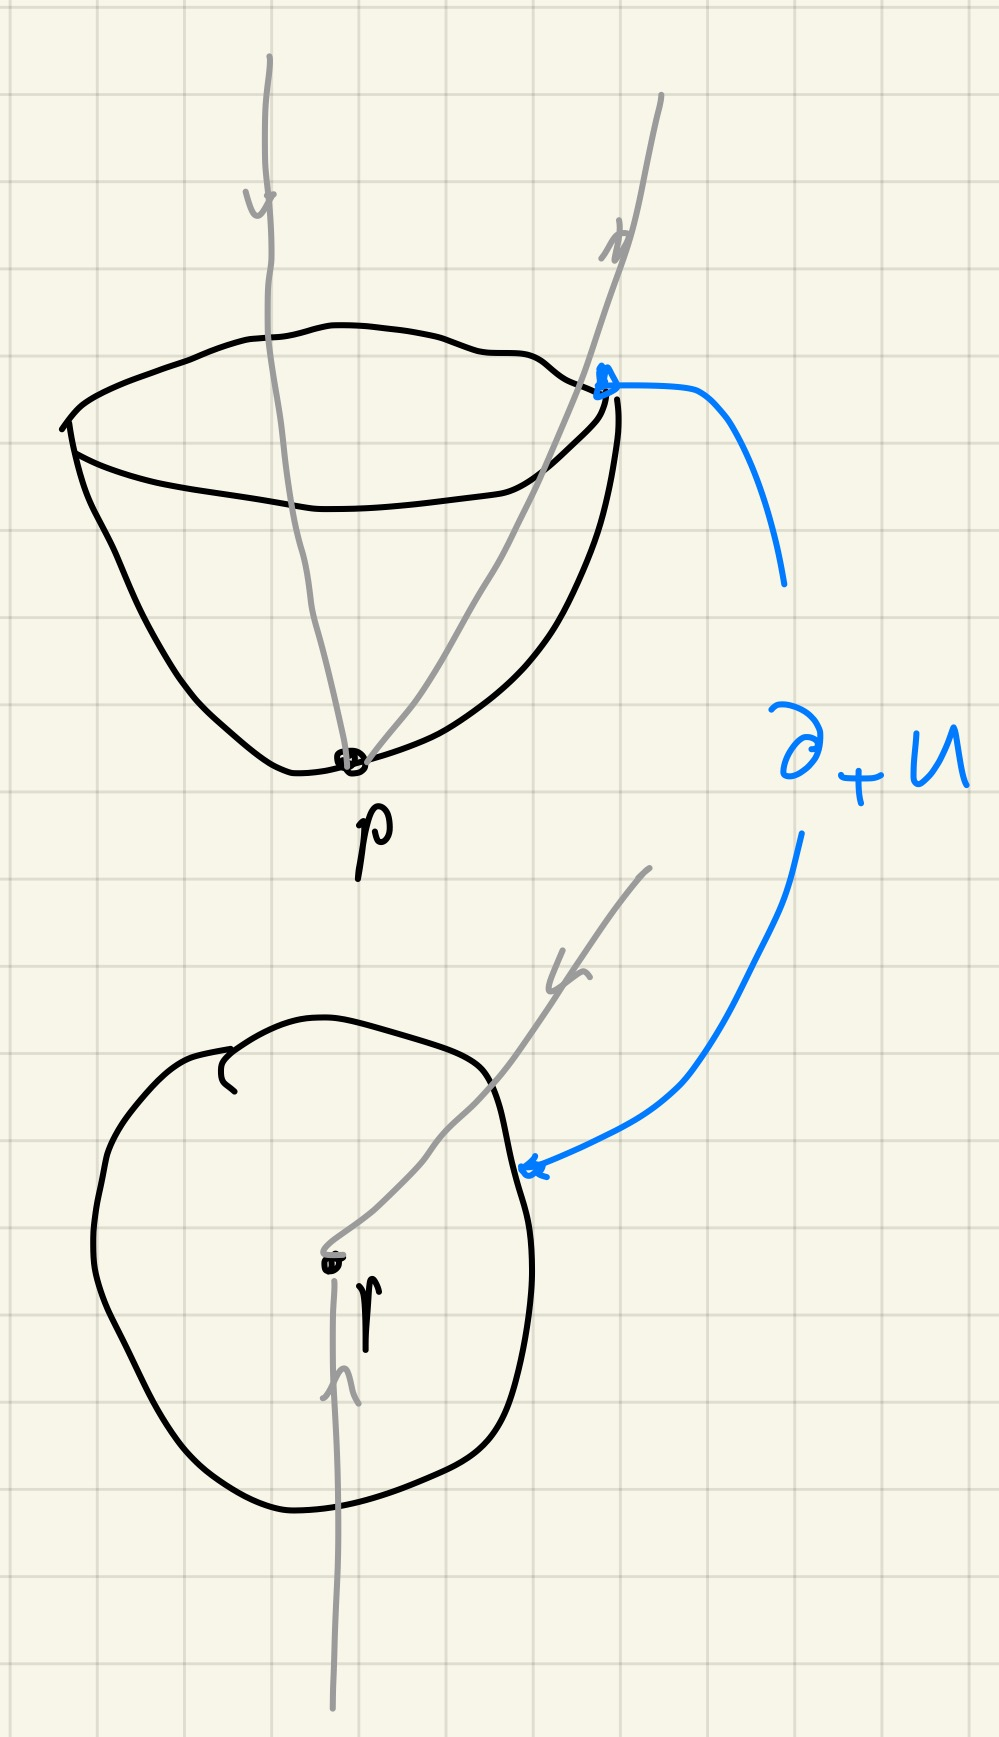
\includegraphics[width=.4\linewidth]{../resources/def-notation-morse-umgebung-1.JPG}
          \captionof{figure}{Index $0$}
          \label{fig: morse umgebung ind 0}
        \end{minipage}%
        \begin{minipage}{.4\textwidth}
          \centering
          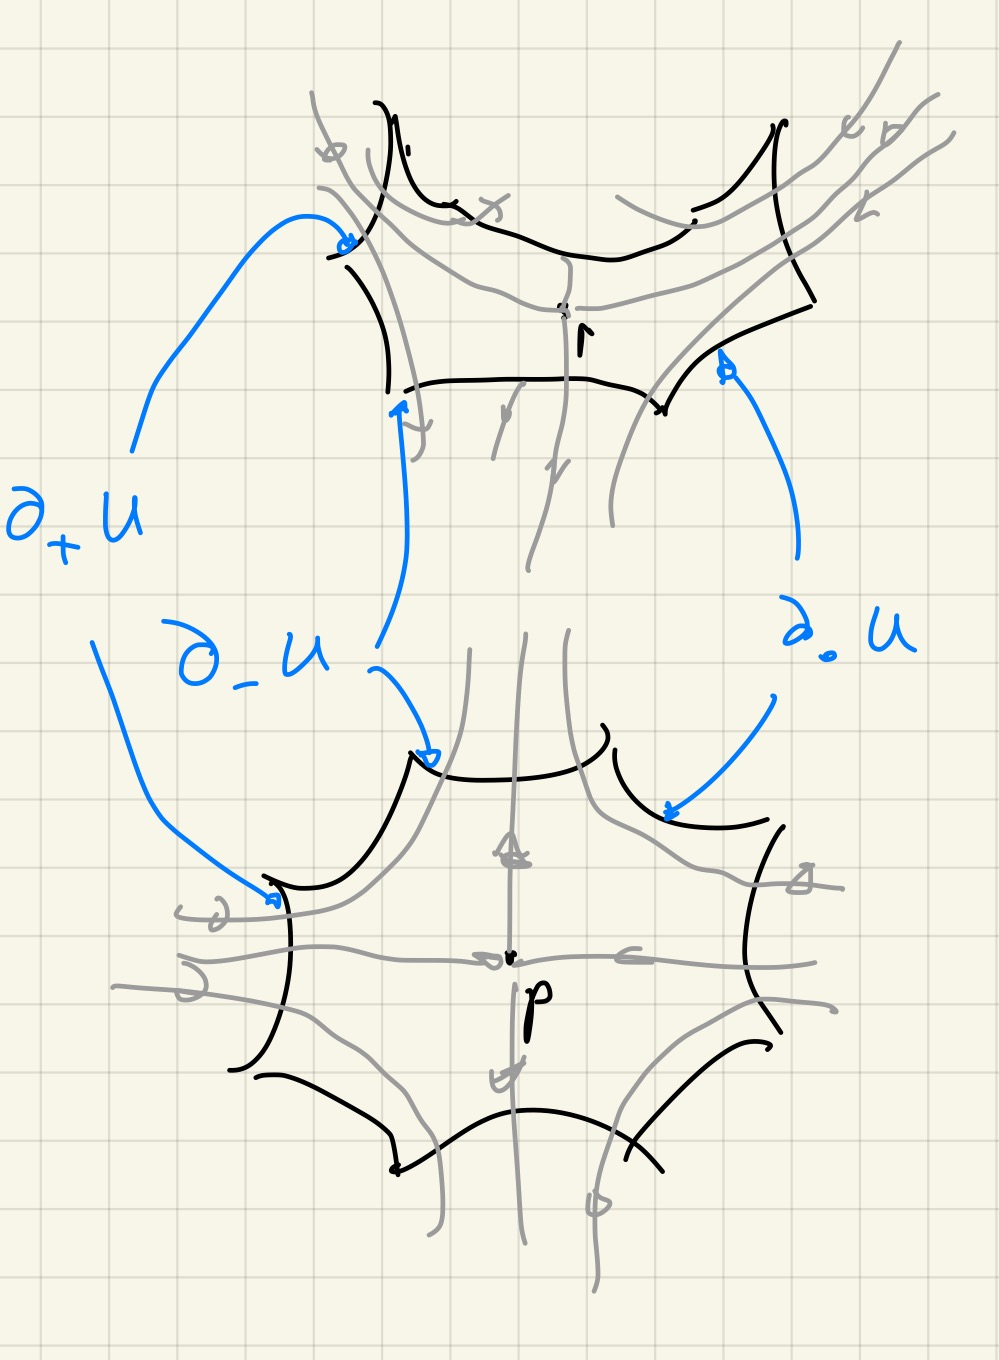
\includegraphics[width=.4\linewidth]{../resources/def-notation-morse-umgebung-2.JPG}
          \captionof{figure}{Index $k$, $0 < k < n$}
          \label{fig: morse umgebung ind k}
        \end{minipage}
    \end{figure}

    $\eps$ und $\eta$ werden häufig in der Notation ausgelassen.
\end{definition}

Mit dieser Vorstellungen von Morse-Funktinoen können wir die folgende Aussage beweisen.

\begin{prop}
    Ist $f \colon M \to \R$ eine Morse Funktion und $p$ ein kritischer Punkt von $f$, dann sind
    $\stab (p)$ und $\unst (p)$ Mannigfaltigkeiten mit 
    \[ \dim \unst (p) = n - \dim \stab (p) = \Index (p) \]
\end{prop}

\begin{proof}
    Es sei $(\psi, V)$ eine Morse Karte um $p$ und $\Omega(p) \subseteq V$ in einer Form wie 
    in ~\ref{def: notation morse umgebung}. Es sei außerdem $\phi$ der Fluss eines 
    Pseudo-Gradientenfeldes von $f$. Dann ist 
    \[ \Phi \colon \del_+ \Omega (p) \cap \stab (p) \times \R \to M ; \; \Phi (q, t) = \phi_t(q) \]
    eine Einbettung und es gilt 
    \[ \stab (p) = \Ima \Phi \cup \psi^{-1}(U \cap V_+) . \]
    Tatsächlich ist 
    \[ \stab (p) - \Ima \Phi = \{ p \} , \]
    denn $\lim_{t \to \infty} \phi_t(q) = p$ für $q \in \del_+ \Omega (p) \cap \stab (p)$. 
    Außerdem ist 
    \[ \del_+ U \cap V_+ = \{ x \in \R^n: \| x_+ \|^2 = \eps \} \diffeo S^{n - k - 1} , \] 
    denn für alle $x \in V_+$ gilt sowieso schon $x_- = 0$. Also ist $\stab(p)$ diffeomorph zum Raum 
    $S^{n - k - 1} \times (-\infty, \infty]/\sim$, in dem alle Punkte in $\infty$ zusammengeklebt 
    werden. Dieser Quotient ist wiederum diffeomorph zur offenen Kreisscheibe mit Dimension $n - k$.
    Genauso zeigt man, dass $\unst (p)$ diffeomorph zur offenen Kreisscheibe mit Dimension $k$ ist.
\end{proof}

\begin{prop}
    \label{prop: trajektorien enden in kritischen punkten}
    Es sei $f \colon M \to \R$ eine Morse-Funktion und $X$ ein Pseudo-\\Gradientenfeld von $f$. 
    Sei außerdem $M$ kompakt. Ist dann $\phi$ der Fluss von $X$, dann existieren für jeden Punkt 
    $p \in M$ kritische Punkte $q$ und $r$ von $f$, sodass
    \[ \lim_{t \to + \infty} \phi_t(p) = q \;\;\; 
    \text{ und } \;\;\; \lim_{t \to -\infty} \phi_t(p) = r \]
\end{prop}

\begin{proof}
    Wir zeigen die erste Aussage. Seien für jeden kritischen Punkt $p$ $(U_p, \psi_p)$ Morse Karten.
    Es ist $\lim_{t \to + \infty} \phi_t(q) = p$, genau dann wenn
    der Fluss $\phi_{\bullet}(q)$ den Punkt $q$ irgendwann in die Umgebung 
    $\del_+ \Omega (p) \cap \stab(p)$ transportiert. Angenommen $\phi_{\bullet}(q)$ transportiert
    $q$ nie zu einem kritischen Punkt. Jedes mal wenn $\phi_{\bullet}(q)$ also ins Innere einer
    Morse-Umgebung $U_q$ gerät, muss diese Umgebung auch wieder verlassen werden. Da 
    $f \circ \phi_{bullet}(q)$ monoton ist, kann nachdem $\phi_{bullet}(q)$ die Morse-Umgebung 
    $\Omega (p)$ verlassen hat, nie wieder zu dieser zurückgekehrt werden.
    Sei also 
    \[ \Omega = \bigcup_{p \in \Crit(f)} \Omega (p) \]
    und $t_0$ der Zeitpunkt an dem $\phi_{\bullet} (q)$ die Umgebung $\Omega$ das letzte mal verlässt.
    Da $M - \Omega$ keine kritischen Punkte von $f$ enthält existiert ein $\eps_0 > 0$, sodass für 
    alle $x \in M - U$ gilt 
    \[ \opd f (x) ((X(x))) \leq - \eps_ . \]
    Wir rechnen also: Für jedes $t \geq t_0$ gilt
    \begin{align*}
        f(\varphi_t(q) - f(\varphi_{t_0}(q))) = & 
            \int_{t_0}^t \derive[f \circ \phi_{\bullet}(q)]{s} (s) \opd s \\
        = & \int_{t_0}^t \opd f (\phi_s(q)) (X(\phi_s(q))) \opd s \\
        \leq & - \eps_0 (t - t_0) . 
    \end{align*}
    Also für $t \to + \infty$ gilt $f(\phi_t(p)) \to - \infty$. Das kann aber nicht sein, denn da 
    $M$ kompakt ist und $\R$ Hausdorff, ist $f$ eigentlich, also ist $\Ima f$ kompakt. 
    \todo{stimmt das?} Also kann $\phi_{\bullet}(p)$ 
    nicht alle $U_q$ verlassen. aber dann ist 
    \[ \lim_{t \to + \infty} \phi_t(q) = p \]
    für einen kritischen Punkt $p$.
    Genauso zeigt man, dass $\lim_{t \to - \infty} \phi_t(p) = r$ für einen kritischen Punkt $r$.
\end{proof}

\begin{definition}[Smale-Bedingung]
    \label{def: smale-bedingung}
    Es sei $M$ eine Mannigfaltigkeit und $U$ und $V$ Untermannigfaltigkeiten von $M$. Wir sagen 
    $U$ und $V$ sind \textit{transversal} und schreiben $U \pitchfork V$, falls für alle Punkte 
    $p \in U \cap V$ gilt 
    \[ T_pU + T_pV = T_pM . \]
    Ein Vektorfeld $X \in \VFs (M)$ heißt \textit{transversal} zur Untermannigfaltigkeit $U$, falls 
    für alle $p$ in $U$ gilt 
    \[ \langle X(p) \rangle + T_pU = T_pM . \]

    Sei nun $f \colon M \to \R$ eine Morse Funktion und $X$ ein Pseudo-Gradientenfeld von $f$. Dann sagen
    wir, dass $X$ die \textit{Smale-Bedingung} erfüllt, falls für alle kritischen Punkte $p$ und $q$ von 
    $f$ gilt 
    \[ \stab (p) \pitchfork \unst (q) . \]
    Ein Paar $(f, X)$ aus einer Morse-Funktion $f$ und einem Pseudo-Gradientenfeld $X$, das die 
    Smale-Bedingung erfüllt, nennt man \textit{Morse-Smale Paar}.
\end{definition}

\begin{prop}
    \label{prop: schnitt von transversalen untermannigfaltigkeiten}
    Sind $U_1$ und $U_2$ Untermannigfaltigkeiten von einer $n$-\\
    dimensionalen Mannigfaltigkeit $M$ mit 
    Dimensionen $d_1$ und $d_2$, sodass 
    \[ U_1 \pitchfork U_2 , \]
    dann ist $U_1 \cap U_2$ eine Untermannigfaltigkeit von $M$ mit Dimension $d_1 + d_2 - n$.
\end{prop}

\begin{proof}
    Es sei $p \in U_1 \cap U_2$. Da $U_1$ und $U_2$ Untermannigfaltigkeiten sind existieren 
    Karten $(\phi_1, V_1)$ und $(\phi_2, V_2)$ von $M$, sodass 
    \[ \phi_1 = (\phi_1', \phi_1'') \colon V_1 \to 
        \Omega_1 \times \Omega_1' \subseteq \R^{d_1} \times \R^{n - d_1} \]
    mit $\phi_1(V_1 \cap U_1) = \Omega_1 \times \{ 0 \}$ und 
    \[ \phi_2 = (\phi_2', \phi_2'')\colon V_2 \to 
        \Omega_2 \times \Omega_2' \subseteq \R^{d_2} \times \R^{n - d_2} \]
    mit $\phi_2(V_2 \cap U_2) = \Omega_2 \times \{ 0 \}$. Definiere 
    \[ \phi'' = (\phi_1'', \phi_2'') \colon 
        M \supseteq V_1 \cap V_2 \to \R^{n - d_1} \times \R^{n - d_2}. \]
    Dann ist 
    $(\phi'')^{-1}(0) = (U_1 \cap V_1) \cap (U_2 \cap V_2) = (U_1 \cap U_2) \cap (V_1 \cap V_2) := V$.
    Wir wollen nun den Satz über reguläre Werte anwenden, aber dafür müssen wir zeigen, dass 
    $\opd \phi'' (p)$ surjektiv ist. Bemerke, dass 
    $\opd \phi'' (p) = \opd (\phi''_1, \phi''_2) (p) = (\opd \phi''_1 (p), \opd \phi''_2 (p))$.
    Es sei $v \in T_p \R^{n - d_1}$ und $w \in T_p\R^{n - d_2}$. Da $\opd \phi''_1 (p)$ und 
    $\opd \phi''_2 (p)$ surjektiv sind, und da $U_1$ und $U_2$ transversal sind, 
    existieren $v_1' + v_2', w_1' + w_2' \in T_pU_1 + T_pU_2$, sodass 
    $\opd \phi''_1 (p) (v_1 + v_2) = \opd \phi''_1 (p) (v_2) = v$ und 
    $\opd \phi''_2 (p) (w_1 + w_2) = \opd \phi''_2 (p) (w_1) = w$.
    Die ersten Gleichheiten gelten, da $T_p U_1$ der Kern von $\opd \phi''_1 (p)$ und 
    $T_p U_2$ der Kern von $\opd \phi''_2 (p)$ sind. Dann gilt
    \[ \opd \phi'' (p) (w_1' + v_2')  = 
        ( \opd \phi''_1 (p) (v_2'), \opd \phi''_2 (p) (w_1')) = (v, w) . \]
    Wir können also den Satz über reguläre Werte anwenden, dann ist $V$ eine Untermannigfaltigkeit
    mit Dimension $n - ((n - d_1) + (n - d_2)) = d_1 + d_2 - n$. Dann ist auch $U_1 \cap U_2$
    eine Untermannigfaltigkeit von Dimension $d_1 + d_2 - n$.
\end{proof}

Dann folgt direkt:

\begin{prop}
    Es sei $f \colon M \to \R$ eine Morse Funktion und $p$ und $q$ kritische Punkte von mit Index $k_1$
    und $k_2$ respektive. Falls $X$ die Smale-Bedingung erfüllt ist
    \[ \mathcal{M} (p, q) := \unst (p) \cap \stab (q) = 
        \left\{ r \in M : \lim_{t \to - \infty} \phi_t(p) \text{ und } 
        \lim_{t \to + \infty} \phi_t(q) \right\} \]
    ist eine Mannigfaltigkeit mit Dimension $k_1 - k_2$.
\end{prop}

Der Raum $\mathcal{M} (p, q)$ beinhaltet alle Punkte, die auf Trajektorien zwischen den kritischen
Punkten $p$ und $q$ liegen. 

\todo{Zeichnung}

\begin{prop}
    \label{prop: wohldefiniertheit von Lt}
    $\R$ wirkt via $(p, t) \mapsto \phi_t(p)$ auf $\mathcal{M}(p, q)$. Sind $p$ und $q$ kritische 
    Punkte mit $p \neq q$ und Indizes $k_1$ und $k_2$, dann ist 
    \[ \Lt (p, q) = \mathcal{M} (p, q) / \R \]
    eine $k_1 - k_2 - 1$-dimensionale Mannigfaltigkeit und es gilt 
    \[ \Lt (p, q) \diffeo \mathcal{M} (p, q) \cap f^{-1}(c) \]
    für einen regulären Wert $c$ zwischen $f(p)$ und f(q)
    (Wir können ohne Beschränkung der Allgemeinheit annehmen, dass $f(p) \neq f(q)$).
\end{prop}

\begin{proof}
    Die Gruppenwirkung ist frei, denn in $\mathcal{M} (p, q)$
    sind keine kritischen Punkte, da $p \neq q$. Es sei $x$ in $\mathcal{M} (p, q)$. 
    Ist nun $t \neq 0$, dann gilt da $f \circ \phi_{\bullet}(x)$ streng monoton ist 
    $f(\phi_t(x)) \neq f(\phi_0(x)) = f(x)$, also $\phi_t(x) \neq x$.

    Es sei nun $c$ ein regulärer Wert zwischen $f(p)$ und $f(q)$. $f^{-1}(c)$ ist eine 
    $n - 1$-dimensionale Mannigfaltigkeit, und für das Pseudo-Gradientenfeld $X$ gilt 
    $X \pitchfork f^{-1}(c)$, und da für jeden Punkt $a$ gilt $X(a) \in T_a \mathcal{M} (p, q)$
    ist $f^{-1}(c) \cap \mathcal{M} (p, q)$ eine $k_1 - k_2 - 1$-dimensionale Mannigfaltigkeit.
    Sei 
    \[ \iota \colon \mathcal{M} (p, q) \cap f^{-1}(c) \to \mathcal{M}(p, q)\] 
    die Inklusion und 
    \[ p \colon \mathcal{M} (p, q) \to \Lt (p, q) \] 
    die Quotientenabbildung. $p \circ \iota$ ist bijektiv und stetig, und ist 
    $U \subseteq \mathcal{M} (p, q)$ offen, dann ist $p \circ \iota (U)$ offen in $\Lb (p, q)$. 
    Also ist $p \circ \iota$ ein Homeomorphismus und $\Lt (p, q)$ ist Hausdorff, also ist $\Lt (p, q)$
    eine Mannigfaltigkeit, und es gilt sogar
    \[ \Lt (p, q) \diffeo \mathcal{M} (p, q) \cap f^{-1}(c) \]
\end{proof}

Der Raum $\Lt (p, q)$ enthält für jede Trajektorie, die zwischen den kritischen Punkten $p$ und $q$ 
verläuft einen Repräsentanten. Später wird $\Lt (p, q)$ benutzt, um den Morse-Komplex zu definieren.
Die Smale Bedingung ist also für unsere Zwecke wichtig.

Wir gewinnen auch eine wichtige Erkenntnis: 

\begin{corollary}
    Der Index von kritischen Punkten verringert sich entlang von Trajektorien. Denn falls 
    $\Index (p) \leq \Index (q)$, dann ist die Dimension von $\Lt (p, q)$
    kleiner $0$, also ist dann $\Lt (p, q) = \varnothing$.
\end{corollary}

Um den Morse Komplex für jede (kompakte) Mannigfaltigkeit definieren zu können, muss noch gezeigt
werden, dass auf jeder Mannigfaltigkeit tatsächlich ein Morse-Smale Paar existiert. 
Sogar noch stärker ist die folgende Aussage:

\begin{theorem}[Satz von Smale-Kupta]
    Es sei $M$ eine Mannigfaltigkeit mit Rand und $f$ eine Morse-Funktion. Es sei $\Omega$ die 
    Vereinigung von Morse-Umgebungen von allen kritischen Punkten. Sei $X$ ein Pseudo-Gradientenfeld 
    von $f$. Dann existiert ein Pseudo-Gradientenfeld $X'$ von $f$, das die Smale Bedingung erfüllt, 
    das innerhalb von $\Omega$ gleich $X$ ist und für das gilt:

    Für jedes $\eps > 0$, jeden Atlas $(\phi_i, U_i)_{i \in I}$ von $M$ und alle $i \in I$ existiert 
    für jede Kompakte Teilmenge $K_i \subseteq U_i$ ein Vektorfeld $X'$, sodass 
    \[ \| \opd \phi_i^{-1} (\cdot) (X') - \opd \phi_i^{-1} (\cdot) (X) \| < \eps . \]
\end{theorem}

\begin{proof}
    Der Satz wurde von S. Smale in \cite{smale1} bewiesen.
\end{proof}